\documentclass[11pt]{article}
\usepackage[utf8]{inputenc}
\usepackage[T1]{fontenc}
\usepackage{amsmath}
\usepackage{amssymb}
\usepackage{multicol}
\usepackage{geometry}
\usepackage{tikz}
\usepackage{enumitem}
\usepackage{xcolor}
\usepackage{titlesec}
\usepackage{tcolorbox} % <<-- necessário para as caixas coloridas
\tcbset{enhanced, boxrule=0.8pt, arc=4pt, auto outer arc} 

% Configurações de layout
\geometry{a4paper, left=1cm, right=1cm, top=0.5cm, bottom=1.2cm}
\setlength{\columnseprule}{0.4pt}

% Cores para títulos
\titleformat{\section}{\normalfont\Large\bfseries\color{blue}}{\thesection}{1em}{}
\titleformat{\subsection}{\normalfont\large\bfseries\color{red}}{\thesubsection}{1em}{}

\title{\textcolor{orange}{Terceiro Trimestre: Matemática
    \\Progressão Aritmética - Revisão}}
\author{Professor: Jefferson}
\date{}

\begin{document}

\maketitle
\vspace{-1cm}

%\begin{center}
%\large{Nome: \underline{\hspace{8cm}} \quad Turma: \underline{\hspace{3cm}}}
%\end{center}

\begin{multicols}{2}

\section*{Fórmulas Importantes}

\subsection*{Termo Geral da PA}

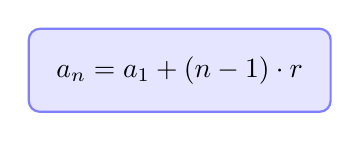
\begin{tikzpicture}
\node[rectangle, fill=blue!10, rounded corners, inner sep=10pt, draw=blue!50, thick] (box) {
$\displaystyle a_n = a_1 + (n-1) \cdot r$
};
\end{tikzpicture}

\textbf{Onde:}
\begin{itemize}
\item $a_n$ = termo que queremos
\item $a_1$ = primeiro termo
\item $n$ = posição do termo
\item $r$ = razão (diferença entre termos)
\end{itemize}

\subsection*{Razão da PA}

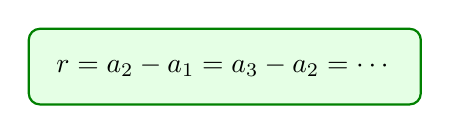
\begin{tikzpicture}
\node[rectangle, fill=green!10, rounded corners, inner sep=10pt, draw=green!50!black, thick] (box) {
$\displaystyle r = a_2 - a_1 = a_3 - a_2 = \cdots$
};
\end{tikzpicture}

\subsection*{Soma dos Termos}

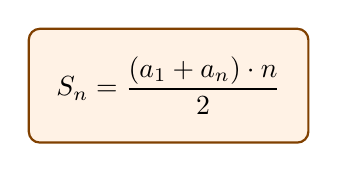
\begin{tikzpicture}
\node[rectangle, fill=orange!10, rounded corners, inner sep=10pt, draw=orange!50!black, thick] (box) {
$\displaystyle S_n = \frac{(a_1 + a_n) \cdot n}{2}$
};
\end{tikzpicture}

\section*{Exercícios Básicos}

\begin{enumerate}[leftmargin=*]

\item Determine a razão de cada PA: 
\begin{enumerate}[label=\alph*)]
\item $(2, 5, 8, 11, \ldots)$
\item $(10, 7, 4, 1, \ldots)$
\item $(-3, 1, 5, 9, \ldots)$
\end{enumerate}

\item Calcule o 5º termo de cada PA:
\begin{enumerate}[label=\alph*)]
\item $(4, 7, 10, 13, \ldots)$
\item $(15, 12, 9, 6, \ldots)$
\item $(1, 4, 7, 10, \ldots)$
\end{enumerate}

\item Encontre o 10º termo das PAs:
\begin{enumerate}[label=\alph*)]
\item $(2, 6, 10, 14, \ldots)$
\item $(20, 17, 14, 11, \ldots)$
\end{enumerate}

\item Escreva os 4 primeiros termos da PA sabendo que:
\begin{enumerate}[label=\alph*)]
\item $a_1 = 3$ e $r = 4$
\item $a_1 = 10$ e $r = -2$
\item $a_1 = -5$ e $r = 3$
\end{enumerate}

\item Calcule a soma dos:
\begin{enumerate}[label=\alph*)]
\item 6 primeiros termos da PA $(1, 3, 5, 7, \ldots)$
\item 8 primeiros termos da PA $(2, 5, 8, 11, \ldots)$
\item 5 primeiros termos da PA $(10, 8, 6, 4, \ldots)$
\end{enumerate}

\item Interpole 3 meios aritméticos entre:
\begin{enumerate}[label=\alph*)]
\item 2 e 10
\item 5 e 17
\end{enumerate}

\item Problemas simples:
\begin{enumerate}[label=\alph*)]
\item Uma PA tem $a_1 = 4$ e $r = 3$. Qual é o 8º termo?
\item Uma PA tem $a_1 = 20$ e $r = -2$. Qual é o 6º termo?
\item Calcule a soma dos 10 primeiros termos da PA $(1, 4, 7, 10, \ldots)$
\end{enumerate}

\item Complete as PAs:
\begin{enumerate}[label=\alph*)]
\item $( \_, 5, 8, 11, \_ )$
\item $(10, \_, 4, \_, -2)$
\item $( \_, 7, 11, 15, \_ )$
\end{enumerate}

\item Determine o número de termos das PAs:
\begin{enumerate}[label=\alph*)]
\item $(3, 7, 11, \ldots, 43)$
\item $(20, 18, 16, \ldots, -10)$
\end{enumerate}

\item Problemas do cotidiano:
\begin{enumerate}[label=\alph*)]
\item João guarda R\$ 5,00 no 1º dia, R\$ 8,00 no 2º dia, R\$ 11,00 no 3º dia, e assim por diante. Quanto guardará no 10º dia?
\item Uma escada tem degraus com alturas em PA: 20 cm, 25 cm, 30 cm... Qual a altura do 8º degrau?
\end{enumerate}

\end{enumerate}

\section*{Dicas para Resolver}

\begin{itemize}
\item \textbf{Razão}: Sempre subtraia um termo pelo anterior
\item \textbf{Termo geral}: Use $a_n = a_1 + (n-1) \cdot r$
\item \textbf{Soma}: Some primeiro + último, multiplique por n e divida por 2
\item \textbf{Verificação}: Confira se a diferença entre termos é constante
\end{itemize}

% ===========================
% GABARITO COMENTADO EM CAIXAS
% ===========================

\section*{Gabarito}

% Questão 1
\begin{tcolorbox}[colback=blue!8,colframe=blue!60!black, title=\textbf{Questão 1 }, text width=0.9\columnwidth]
Determine a razão de cada PA:

(a)\,$(2,5,8,11,\ldots)$\\ (b) $(10,7,4,1,\ldots)$ \\ (c) $(-3,1,5,9,\ldots)$
\end{tcolorbox}

\begin{tcolorbox}[colback=green!10,colframe=green!60!black, title=\textbf{Solução da questão 1 }, text width=0.9\columnwidth]
\textbf{Definição:} $r = a_2 - a_1$ (diferença entre termos consecutivos).

(a) $r = 5-2 = 3$. \\
Comentário: conferimos $8-5=3$ e $11-8=3$; razão consistente. \\
    \textbf{Resposta (a):} $\boxed{r = 3}$. \\

(b) $r = 7-10 = -3$. \\
Verificação: $4-7=-3$, $1-4=-3$. \\
    \textbf{Resposta (b):} $ \boxed{r = -3}$. \\

(c) $r = 1-(-3) = 4$. \\
Verificação: $5-1=4$, $9-5=4$. \\
    \textbf{Resposta (c):} $\boxed{r = 4}$. 
\end{tcolorbox}

% Questão 2
\begin{tcolorbox}[colback=blue!8,colframe=blue!60!black, title=\textbf{Questão 2 }, text width=0.9\columnwidth]
Calcule o 5º termo de cada PA: \\
(a) $(4,7,10,13,\ldots)$ \\ (b) $(15,12,9,6,\ldots)$ \\ (c) $(1,4,7,10,\ldots)$
\end{tcolorbox}

\begin{tcolorbox}[colback=green!10,colframe=green!60!black, title=\textbf{Solução da questão 2 }, text width=0.9\columnwidth]
Usamos $a_n = a_1 + (n-1)r$ com $n=5$. \\

(a) $r=7-4=3$. \\
$a_5 = 4 + (5-1)\cdot 3 = 4 + 12 = 16$. \\
\textbf{Resposta (a):} $16$. \\

(b) $r=12-15=-3$. \\
$a_5 = 15 + (5-1)\cdot(-3) = 15 -12 = 3$. \\
\textbf{Resposta (b):} $3$. \\

(c) $r=4-1=3$. \\
$a_5 = 1 + 4\cdot 3 = 13$. \\
\textbf{Resposta (c):} $13$.
\end{tcolorbox}

% Questão 3
\begin{tcolorbox}[colback=blue!8,colframe=blue!60!black, title=\textbf{Questão 3 }, text width=0.9\columnwidth]
Encontre o 10º termo das PAs: \\
(a) $(2,6,10,14,\ldots)$ \\ (b) $(20,17,14,11,\ldots)$
\end{tcolorbox}

\begin{tcolorbox}[colback=green!10,colframe=green!60!black, title=\textbf{Solução da questão 3 }, text width=0.9\columnwidth]
(a) $r=6-2=4$. \\
$a_{10} = 2 + (10-1)\cdot 4 = 2 + 36 = 38$. \\
\textbf{Resposta (a):} $38$. \\

(b) $r=17-20=-3$. \\
$a_{10} = 20 + 9\cdot(-3) = 20 -27 = -7$. \\
\textbf{Resposta (b):} $-7$. \\
\end{tcolorbox}

% Questão 4
\begin{tcolorbox}[colback=blue!8,colframe=blue!60!black, title=\textbf{Questão 4 }, text width=0.9\columnwidth]
Escreva os 4 primeiros termos da PA sabendo que: 

(a) $a_1=3, r=4$ \\ (b) $a_1=10, r=-2$ \\ (c) $a_1=-5, r=3$
\end{tcolorbox}

\begin{tcolorbox}[colback=green!10,colframe=green!60!black, title=\textbf{Solução da questão 4 }, text width=0.9\columnwidth]
(a) $a_1=3$; $a_2=3+4=7$; $a_3=7+4=11$; $a_4=11+4=15$. \\
\textbf{Resposta (a):} $(3,7,11,15)$. \\

(b) $a_1=10$; $a_2=8$; $a_3=6$; $a_4=4$. (subtraindo 2 a cada passo) \\
\textbf{Resposta (b):} $(10,8,6,4)$. \\

(c) $a_1=-5$; $a_2=-2$; $a_3=1$; $a_4=4$. \\
\textbf{Resposta (c):} $(-5,-2,1,4)$. \\
\end{tcolorbox}

% Questão 5
\begin{tcolorbox}[colback=blue!8,colframe=blue!60!black, title=\textbf{Questão 5 }, text width=0.9\columnwidth]
Calcule a soma dos: \\
(a) 6 primeiros termos da PA $(1,3,5,7,\ldots)$ \\
(b) 8 primeiros termos da PA $(2,5,8,11,\ldots)$ \\
(c) 5 primeiros termos da PA $(10,8,6,4,\ldots)$
\end{tcolorbox}

\begin{tcolorbox}[colback=green!10,colframe=green!60!black, title=\textbf{Solução da questão 5 }, text width=0.9\columnwidth]

Usamos $S_n = \dfrac{(a_1 + a_n)\, n}{2}$. \\

    (a) PA com $a_1=1$, $r=2$. Primeiro encontramos $a_6$, pela fórmula temos $\boxed{a_6 = 1 + 5\cdot2 = 11}$. \\

$S_6 = \dfrac{(1+11)\cdot 6}{2} = \dfrac{12\cdot6}{2}=36$. \\
\textbf{Resposta (a):} $36$. \\

(b) $a_1=2$, $r=3$. $a_8 = 2 + 7\cdot3 = 23$. \\
$S_8 = \dfrac{(2+23)\cdot8}{2} = \dfrac{25\cdot8}{2}=100$. \\
\textbf{Resposta (b):} $100$. \\

(c) $a_1=10$, $r=-2$. $a_5 = 10 + 4\cdot(-2) = 10 -8 = 2$. \\
$S_5 = \dfrac{(10+2)\cdot5}{2} = \dfrac{12\cdot5}{2} = 30$. \\
\textbf{Resposta (c):} $30$.
\end{tcolorbox}

% Questão 6
\begin{tcolorbox}[colback=blue!8,colframe=blue!60!black, title=\textbf{Questão 6 }, text width=0.9\columnwidth]
Interpole 3 meios aritméticos entre: \\
(a) 2 e 10 \quad (b) 5 e 17
\end{tcolorbox}

\begin{tcolorbox}[colback=green!10,colframe=green!60!black, title=\textbf{Solução da questão 6 }, text width=0.9\columnwidth]
Interpolar 3 meios aritméticos significa inserir 3 termos entre os dados de modo que a sequência forme uma PA. Assim teremos no total 5 termos: $a_1$, $a_2$, $a_3$, $a_4$, $a_5$ com $a_1$ dado e $a_5$ dado. A razão $r=(a_5-a_1)/4$. \\

(a) $a_1=2$, $a_5=10$ → $r=(10-2)/4 = 8/4 = 2$. \\
Termos: $2,\; 4,\; 6,\; 8,\; 10$. \\
Os 3 meios aritméticos são \(\boxed{4,\;6,\;8}\). \\

(b) $a_1=5$, $a_5=17$ → $r=(17-5)/4 = 12/4 = 3$. \\
Termos: $5,\;8,\;11,\;14,\;17$. \\
Os 3 meios aritméticos são \(\boxed{8,\;11,\;14}\).
\end{tcolorbox}

% Questão 7
\begin{tcolorbox}[colback=blue!8,colframe=blue!60!black, title=\textbf{Questão 7 }, text width=0.9\columnwidth]
Problemas simples: \\
(a) PA com $a_1=4$, $r=3$. Qual o 8º termo? \\
(b) PA com $a_1=20$, $r=-2$. Qual o 6º termo? \\
(c) Soma dos 10 primeiros termos de $(1,4,7,10,\ldots)$
\end{tcolorbox}

\begin{tcolorbox}[colback=green!10,colframe=green!60!black, title=\textbf{Solução da questão 7 }, text width=0.9\columnwidth]
(a) $a_8 = a_1 + 7r = 4 + 7\cdot3 = 4 +21 = 25$. \\
\textbf{Resposta (a):} $25$. \\

(b) $a_6 = 20 + 5\cdot(-2) = 20 -10 = 10$. \\
\textbf{Resposta (b):} $10$. \\
 
(c) Para $(1,4,7,\ldots)$ temos $a_1=1$, $r=3$. $a_{10} = 1 + 9\cdot3 = 28$. \\
$S_{10} = \dfrac{(a_1 + a_{10})\cdot 10}{2} = \dfrac{(1+28)\cdot10}{2} = \dfrac{29\cdot10}{2} = 145$. \\
\textbf{Resposta (c):} $145$.
\end{tcolorbox}

% Questão 8
\begin{tcolorbox}[colback=blue!8,colframe=blue!60!black, title=\textbf{Questão 8 }, text width=0.9\columnwidth]
Complete as PAs: \\
(a) $(\_,5,8,11,\_)$ \\ (b) $(10,\_,4,\_,-2)$ \\ (c) $(\_,7,11,15,\_)$
\end{tcolorbox}

\begin{tcolorbox}[colback=green!10,colframe=green!60!black, title=\textbf{Solução da questão 8 }, text width=0.9\columnwidth]
(a) Observando 5,8,11 → diferença $r=3$. Então termos são: $2,5,8,11,14$. \\
\textbf{Resposta (a):} $(2,5,8,11,14)$. \\

(b) Temos $10, \_, 4, \_, -2$. Os passos entre 10 e -2: distância total $-2-10=-12$ em 4 intervalos → $r=-12/4=-3$. \\
Complete: $10,7,4,1,-2$. \\
\textbf{Resposta (b):} $(10,7,4,1,-2)$. \\

(c) Dados 7,11,15 → $r=4$. Os termos colocados: $3,7,11,15,19$. \\
\textbf{Resposta (c):} $(3,7,11,15,19)$.
\end{tcolorbox}

% Questão 9
\begin{tcolorbox}[colback=blue!8,colframe=blue!60!black, title=\textbf{Questão 9 }, text width=0.9\columnwidth]
Determine o número de termos das PAs: \\
(a) $(3,7,11,\ldots,43)$ \quad (b) $(20,18,16,\ldots,-10)$
\end{tcolorbox}

\begin{tcolorbox}[colback=green!10,colframe=green!60!black, title=\textbf{Solução da questão 9 }, text width=0.9\columnwidth]
Usamos fórmula do termo: $a_n = a_1 + (n-1)r$. Isolamos $n$.\\

(a) $a_1=3$, $r=4$, queremos $a_n=43$. \\
$43 = 3 + (n-1)\cdot4 \Rightarrow 40 = 4(n-1) \Rightarrow n-1=10 \Rightarrow n=11$. \\
\textbf{Resposta (a):} $11$ termos. \\

(b) $a_1=20$, $r=-2$, $a_n = -10$. \\
$-10 = 20 + (n-1)(-2) \Rightarrow -30 = -2(n-1) \Rightarrow n-1 = 15 \Rightarrow n=16$. \\
\textbf{Resposta (b):} $16$ termos.
\end{tcolorbox}

% Questão 10
\begin{tcolorbox}[colback=blue!8,colframe=blue!60!black, title=\textbf{Questão 10 }, text width=0.9\columnwidth]
Problemas do cotidiano: \\
(a) João guarda R\$5,00 no 1º dia, R\$8,00 no 2º dia, R\$11,00 no 3º dia, ... Quanto guardará no 10º dia? \\
(b) Degraus: 20 cm, 25 cm, 30 cm... Qual a altura do 8º degrau? \\
\end{tcolorbox}

\begin{tcolorbox}[colback=green!10,colframe=green!60!black, title=\textbf{Solução da questão 10 }, text width=0.9\columnwidth]
Ambos são PAs com $r=3$.

(a) $a_1=5$, $r=3$. $a_{10} = 5 + 9\cdot3 = 5 +27 = 32$. \\
\textbf{Resposta (a):} R\$ \(\mathbf{32,00}\). \\

(b) $a_1=20$, $r=5$. $a_8 = 20 + 7\cdot5 = 20 +35 = 55\) cm. \\
\textbf{Resposta (b):} \(\mathbf{55\ \text{cm}}\).
\end{tcolorbox}

\end{multicols}

\end{document}

